\documentclass[11pt,a4paper]{scrartcl}
\usepackage[utf8]{inputenc}
\usepackage[utf8]{inputenc}
\usepackage[ngerman]{babel}
\usepackage[T1]{fontenc}
\usepackage{amsmath}
\usepackage{amsfonts}
\usepackage{amssymb}
\usepackage{mathtools}
\usepackage{graphicx}
\usepackage{multirow}
\usepackage{fancyhdr}
\usepackage{float}
\pagestyle{fancy}
\usepackage[a4paper,
			bottom=1.7in,
			left=1.2in,
			right=1.2in,
			top=1.2in,
			headsep = 35pt]
	{geometry}
\usepackage{tikz}% for drawing automata etc
\usetikzlibrary{automata,arrows,chains,shapes.misc,scopes,petri,matrix,patterns}
%\usepackage[x11names]{xcolor}
%\usepackage[parfill]{parskip}
\usepackage{array}
%\usepackage{gslist}
%\usepackage{subfigure}
\usepackage{subcaption}
\usepackage{enumitem}
\usepackage{algpseudocode} %for pseudocode
\usepackage[siunitx,european,straightlabels,straightvoltages]{circuitikz} %draw Electrical Circuits
\usepackage[miktex]{gnuplottex}
\usepackage{pgfplots}
\usepackage{bm} %Bold Math

\ctikzset{bipoles/text rotate/.initial=0,% <=new key
rotation/.style={\circuitikzbasekey/bipoles/text rotate=#1},% style for ease introduction in code
}

% code from pgfcircbipoles.sty
\makeatletter
\pgfcircdeclarebipole{}{\ctikzvalof{bipoles/ammeter/height}}{ammeter}{\ctikzvalof{bipoles/ammeter/height}}{\ctikzvalof{bipoles/ammeter/width}}{
    \def\pgf@circ@temp{right}
    \ifx\tikz@res@label@pos\pgf@circ@temp
        \pgf@circ@res@step=-1.2\pgf@circ@res@up
    \else
        \def\pgf@circ@temp{below}
        \ifx\tikz@res@label@pos\pgf@circ@temp
            \pgf@circ@res@step=-1.2\pgf@circ@res@up
        \else
            \pgf@circ@res@step=1.2\pgf@circ@res@up
        \fi
    \fi

    \pgfpathmoveto{\pgfpoint{\pgf@circ@res@left}{\pgf@circ@res@zero}}       
    \pgfpointorigin \pgf@circ@res@other =  \pgf@x  \advance \pgf@circ@res@other by -\pgf@circ@res@up
    \pgfpathlineto{\pgfpoint{\pgf@circ@res@other}{\pgf@circ@res@zero}}
    \pgfusepath{draw}

    \pgfsetlinewidth{\pgfkeysvalueof{/tikz/circuitikz/bipoles/thickness}\pgfstartlinewidth}

        \pgfscope
            \pgfpathcircle{\pgfpointorigin}{\pgf@circ@res@up} % change this if you want to touch the wires
            \pgfusepath{draw}       
        \endpgfscope    

    \pgftransformrotate{\ctikzvalof{bipoles/text rotate}}% <= magic line
    \pgfsetlinewidth{\pgfstartlinewidth}

    \pgfsetarrowsend{latex}
    \pgfpathmoveto{\pgfpoint{\pgf@circ@res@other}{\pgf@circ@res@down}}
    \pgfpathlineto{\pgfpoint{-1.06\pgf@circ@res@other}{1.06\pgf@circ@res@up}} % change this if you want to touch the wires
    %\pgfusepath{draw} % comment this if you don't need the diagonal arrow
    \pgfsetarrowsend{}


    \pgfpathmoveto{\pgfpoint{-\pgf@circ@res@other}{\pgf@circ@res@zero}}
    \pgfpathlineto{\pgfpoint{\pgf@circ@res@right}{\pgf@circ@res@zero}}
    %\pgfusepath{draw} % comment this if you don't need the diagonal arrow


    \pgfnode{circle}{center}{\textbf{A}}{}{}
}

% code from pgfcircbipoles.sty
\pgfcircdeclarebipole{}{\ctikzvalof{bipoles/voltmeter/height}}{voltmeter}{\ctikzvalof{bipoles/voltmeter/height}}{\ctikzvalof{bipoles/voltmeter/width}}{
    \def\pgf@circ@temp{right}
    \ifx\tikz@res@label@pos\pgf@circ@temp
        \pgf@circ@res@step=-1.2\pgf@circ@res@up
    \else
        \def\pgf@circ@temp{below}
        \ifx\tikz@res@label@pos\pgf@circ@temp
            \pgf@circ@res@step=-1.2\pgf@circ@res@up
        \else
            \pgf@circ@res@step=1.2\pgf@circ@res@up
        \fi
    \fi

    \pgfpathmoveto{\pgfpoint{\pgf@circ@res@left}{\pgf@circ@res@zero}}       
    \pgfpointorigin \pgf@circ@res@other =  \pgf@x  \advance \pgf@circ@res@other by -\pgf@circ@res@up
    \pgfpathlineto{\pgfpoint{\pgf@circ@res@other}{\pgf@circ@res@zero}}
    \pgfusepath{draw}

    \pgfsetlinewidth{\pgfkeysvalueof{/tikz/circuitikz/bipoles/thickness}\pgfstartlinewidth}

        \pgfscope
            \pgfpathcircle{\pgfpointorigin}{\pgf@circ@res@up} % change this if you want to touch the wires
            \pgfusepath{draw}       
        \endpgfscope    

    \pgftransformrotate{\ctikzvalof{bipoles/text rotate}}% <= magic line
    \pgfsetlinewidth{\pgfstartlinewidth}

    \pgfsetarrowsend{latex}
    \pgfpathmoveto{\pgfpoint{\pgf@circ@res@other}{\pgf@circ@res@down}}
    \pgfpathlineto{\pgfpoint{-1.06\pgf@circ@res@other}{1.06\pgf@circ@res@up}} % change this if you want to touch the wires
    %\pgfusepath{draw} % comment this if you don't need the diagonal arrow
    \pgfsetarrowsend{}


    \pgfpathmoveto{\pgfpoint{-\pgf@circ@res@other}{\pgf@circ@res@zero}}
    \pgfpathlineto{\pgfpoint{\pgf@circ@res@right}{\pgf@circ@res@zero}}
    %\pgfusepath{draw} % comment this if you don't need the diagonal arrow


    \pgfnode{circle}{center}{\textbf{V}}{}{}
}
\makeatother


\author{Alexander Halbarth}

\setlist[enumerate]{label=\alph*)}
%\setlist[itemize]{label=$\rightarrow$}


 \tikzset{
endbox/.style={pattern=crosshatch,minimum height=.8cm}}

%\partfont{\centering}
\newcommand\tab[1][1cm]{\hspace*{#1}}
\usepackage{framed, color}


\newcommand{\UE}{Übung 4}
\newcommand{\name}{Fragenkatalog zum Überprüfungsgespräch Elektrotechnische Grundlagen}
\title{\textbf{Fragenkatalog zum Überprüfungsgespräch Elektrotechnische Grundlagen Übungen für TI 2017 - \UE}}


\newcommand{\ul}[1]{\underline{#1}} % für unterstreichen von einzelnen Symbolen einfach \ul x - wenn man ein Wort unterstrichen will \ul{wort}
%\newcommand\sy[1]{{\underline{\ifmmode\mathtt{#1}\else\texttt{#1}\fi}}} % ähnlich wie \ul - verwendet aber andere Schriftart
%\newlistt\sys\sy{\hspace{1pt}}{}{}{^} % identisch zu \sy, \sys{wort} unterstreicht aber jeden Buchstaben einzeln und \sy{wort} unterstreicht das ganze Wort
% (sofern das Alphabet nur aus einzelnen Zeichen besteht ist \sys{wort} einfacher


%no line indent
\setlength\parindent{0pt}

\fancyhead[R]{\UE}
\fancyhead[L]{\name}
\fancyfoot[C]{\thepage}

\renewcommand{\footrulewidth}{0pt}
\renewcommand{\headrulewidth}{0.5pt}


\begin{document}
\maketitle
\textbf{Frage 1: Was machst Du gerade im Labor und welchen Sinn hat das?}\\
\textbf{Frage 2: Nenne die Grundgrößen der Elektrotechnik, deren Formelzeichen und Einheit.}\\
Spannung $U[$Volt $V]$, Strom $I[$Ampere $A]$, Widerstand $R[$Ohm $\Omega]$,Leistung $P[$Watt $W]$\\
\textbf{Frage 2: Elektrische Spannung: Nenne Definition (nicht über das Ohmsche Gesetz!), Formelzeichen und Einheit}\\
Die potentielle Energie(=Arbeit) die durch eine Ladungstrennung gespeichert wurde.\\
\textbf{Frage 2: Elektrischer Strom: Nenne Definition (nicht über das Ohmsche Gesetz!), Formelzeichen und Einheit}\\
Ladung eines Elektrons $Q_e=1,6 \cdot 10^{-19}C=1,6 \cdot 10^{-19}A\cdot s$\\
$\frac{6*10^{18}e^-}{1s}=\frac{As}{1s} \rightarrow 6 \cdot 10^{18}$ Elektronen fließen durch einen Leiter pro Sekunde bei $1A$\\
\textbf{Frage 2: Elektrischer Widerstand: Nenne Definition (nicht über das Ohmsche Gesetz!), Formelzeichen und Einheit}\\
Ist eine Materialeigenschaft\\
Beispiel Kupfer $17m\Omega \cdot mm^2/m$\\
\textbf{Frage 2: Elektrische Leistung: Nenne Definition, Formelzeichen und Einheit}\\
Die in einer Zeitspannung umgesetzte elektrische Energie bezogen auf die Zeitspanne.\\
\textbf{Frage 2: Wie berechnet man die elektrische Leistung in einem Gleichstromkreis?}\\
$U=R \cdot I \rightarrow P=U \cdot I$\\
\textbf{Berechne die an einem Widerstand entstehende Leistung, wenn durch ihn bei einer Spannung von $2V$ ein Strom von $3A$ fließt.}\\
$6W$\\
\textbf{Frage 2: Welcher Phasenwinkel besteht zwischen Wechselspannung und Wechselstrom an einem idealen Kondensator?}\\
Die Spannung folgt dem Strom um $90^\circ=\pi/2$ nach. (eigentlich $-90^\circ$)\\
\textbf{Welcher Phasenwinkel besteht zwischen Wechselspannung und Wechselstrom an einer idealen Induktivität?\\
(Die Vorzeichen brauchen nicht explizit angegeben zu werden, müssen aber verglichen werden).}\\
Der Strom folgt der Spannung nach um $90^\circ=\pi/2$ nach. (eigentlich $+90^\circ$)\\
\textit{Gehen in entgegengesetzte Richtungen!}\\
\textbf{Frage 2: Formuliere das ohmsche Gesetz.}\\
$U=R*I$\\
\textbf{Berechne den Widerstand, wenn bei einem Strom von $3A$ eine Spannung von $3V$ abfällt.}\\
\textbf{Frage 2: Berechne den Strom, wenn an einem Widerstand von $5\Omega$ eine Spannung von $10V$ abfällt.}\\
\textbf{Frage 2: Berechne die Spannung, wenn durch einen Widerstand von $10\Omega$ ein Strom von $5A$ fließt. }\\
\textbf{Frage 2: Formuliere die Kirchhoffschen Regeln.}\\
\textbf{Auf welchem physikalischen Grundprinzip beruhen diese?}\\
\textit{Energieerhaltung}\\
Maschenregel: Summe aller Spannungen muss 0 ergeben.\\
Knotenregel: Summe aller Ströme muss 0 ergeben.\\
\textbf{An einem Spannungsteiler liegen $9V$. Am oberen Widerstand liegen $6V$ an.}\\
\textbf{Berechne die Spannung am unteren Widerstand.}\\
\textbf{Frage 2: In einen Stromknoten mit drei Leitungen fließen aus einer Leitung $2A$ hinein und aus einer anderen Leitung $3A$ hinein. Was geschieht in der dritten Leitung?}\\
\textbf{Frage 2: Nenne die Zehnerpotenzen zu den SI - Präfixen Nano, Milli und Mikro. Nenne die SI - Präfixe zu: $10^3, 10^6, 10^9$}\\
\begin{tabular}{|l|l|l|}
\hline
\textbf{Präfix} & \textbf{Zeichen} & \textbf{Faktor}\\
\hline\hline
Piko   & p  & $10^{-12}$\\
\hline
Nano   & n  & $10^{-9}$\\
\hline
Mikro  & $\mu$ & $10^{-6}$\\
\hline
Milli  & m  & $10^{-3}$\\
\hline
Zenti  & c  & $10^{-2}$\\
\hline
Dezi   & d  & $10^{-1}$\\
\hline\hline
Deka   & da & $10^{1}$\\
\hline
Hekto  & h  & $10^{2}$\\
\hline
Kilo   & k  & $10^{3}$\\
\hline
Mega   & M  & $10^{6}$\\
\hline
Giga   & G  & $10^{9}$\\
\hline
Tera   & T  & $10^{12}$\\
\hline
\end{tabular}\\
\newpage
\textbf{Frage 3: Ein Sensor hat einen Ausgangswiderstand von $10k\Omega$. Das Signal wird über ein $100m$ langes Koaxialkabel mit einer Kapazität von $100pF/m$ übertragen.}\\
Das Ersatzschaltbild dafür ist ein RC Tiefpass Filter. Die Kapazität ergibt sich durch $100m \cdot 100pF/m=10nF$
\begin{center}
\begin{circuitikz} \draw
			(0,0) to[V<=Sensor,i^>=$I$] (0,2)
						to[R=$10k\Omega$]    (2,2)
						to[C=$10nF$,*-*] (2,0)
						-- (0,0)
						(2,2)--(2.5,2)
						(2,0)--(2.5,0);
\end{circuitikz}
\end{center}
\begin{itemize}
	\item \textbf{Der Sensor liefert ein symmetrisches Rechtecksignal. Schätze die höchste Frequenz dieses Signals ab, das über diese Strecke mit akzeptabler Qualität übertragen werden kann.}\\
				$f_{G}=\dfrac{1}{2 \pi \cdot R \cdot C}=\dfrac{1}{2\pi \cdot 10 \cdot 10}MHz=0,0015 MHz=1,5kHz$\\
				Signale bis zu $0,15kHz$ werden akzeptabel Übertragen.
	\item \textbf{Das Ausgangssignal des Sensors ist ein Sprung von $0.0V$ auf $+3.16V$. Nach welcher Zeit erkennt der Empfänger den Sprung, wenn er bei einer Spannung von etwa $+2.00V$ schaltet.}\\
				$2V$ sind etwa $63\%$ von $3,16V$ daher ist es etwa nach der Zeitkonstante $\tau =R\cdot C=10k \cdot 100 \cdot 100p\;s=100\mu s$
	\item \textbf{Der Sensor liefert ein Sinussignal von etwa $3.3V_{PP}$. Bei welcher Frequenz kommen am Empfänger noch etwa $2.33V_{PP}$ an?}\\
				$20 \cdot log(\dfrac{2,33}{3,3})\approx -3$ \\
				Daraus folgt bei der Grenzfrequenz $f_{G}=\dfrac{1}{2 \pi \cdot R \cdot C}=\dfrac{1}{2\pi \cdot 10 \cdot 10}MHz=0,0015 MHz=1,5kHz$\\
				\textbf{Welche Phasenverschiebung hat das Signal auf seinem Weg durch das Kabel bei dieser Frequenz?} $-45^\circ$
	\item \textbf{Der Sensor liefert ein unsymmetrisches Rechtecksignal: $+10V$ für $100\mu s$, dann $-10V$ für $900\mu s$. Das Signal am Empfänger muss $99\%$ des Sensorsignals sein. Kann dieses Signal über dieses Kabel korrekt übertragen werden?}\\
				Frequenz des Signals $\dfrac{1}{100\mu s + 900\mu s}=1kHz$\\
				$f_{G}=\dfrac{1}{2 \pi \cdot R \cdot C}=\dfrac{1}{2\pi \cdot 10 \cdot 10}MHz=0,0015 MHz=1,5kHz$\\
				Wird nicht genau genug übertragen da größer als $\frac{1}{10}f_G$!
\end{itemize}
\newpage

\textbf{Frage 3: Ein Taster liefert folgendes Signal:} 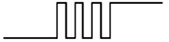
\includegraphics{Taster.png}\\
\textbf{Mit welchem Filter kannst Du dieses Prellen aus dem Signal entfernen?}\\
Tiefpass\\
\textbf{Mit welcher Schaltung kannst Du danach die Flankensteilheit wieder erhöhen?}\\
Schmitt-Trigger

\textbf{Frage 3: Erkläre das Verhalten dieser Schaltung:}\\
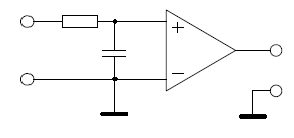
\includegraphics{Schaltung_1.png}\\
Bei hohen Frequenzen lässt lässt der Kondensator immer mehr Spannung durch. Tiefpass Filter\\
OPV als Komperator geschalten. Mögliche Schaltung für Prellreduktion.

\textbf{Frage 3: Skizziere die Übertragungsfunktion dieser Schaltung:\\
(Doppelt logarithmischer Maßstab der Achsen)}\\
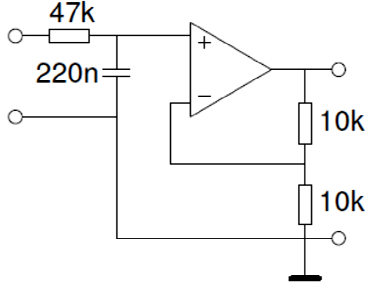
\includegraphics[height=4cm]{Schaltung_2.png}\\
OPV Verstärkung 2-fach$=6dB$\\
$f_G=\dfrac{1}{2 \pi \cdot R \cdot C}=\dfrac{1}{2\pi\cdot 47 \cdot 220}MHz\approx 15Hz$\\
\begin{figure}[H]
	\centering
	\begin{gnuplot}[terminal=pdf,scale=0.8]
			set sample 1000
			set ylabel 'dB'
			set xlabel 'Frequenz'
			set logscale x
			set arrow 1 from 0.01,6 to 15,6 nohead filled lt 1
			set arrow 2 from 15,6 to 1015,-34 nohead filled lt 1
			set arrow 3 from 15,-36 to 15,7 nohead  filled back lw 1 lc rgb "blue
			set label " fg" at 15,0 textcolor rgb "blue"
			plot [0.01:1000] [-36:7] -10000 title 'Schaltung'
	\end{gnuplot}
\end{figure}
\textit{Ab Grenzfrequenz des beschaltenen OPVs Filterverhalten 2. Ordnung}
\newpage

\textbf{Frage 4: Vergleiche das Bode-Diagramm mit einem Spektrum. Was sind die Gemeinsamkeiten?}\\
\textbf{Was wird womit beschrieben?}\\
Beide über Frequenz dargestellt
\begin{itemize}
	\item Bode: Übertragungsfunktion
	\item Spektrum: Stellt Frequenz dar aus dem Signal besteht
\end{itemize}

\textbf{Frage 4: Elektrische Spannung kann unter anderem in $V_{PP}$, $V_{RMS}$ und $dBV_{RMS}$ bzw. $V_{SS}$, $V_{EFF}$ und $dBV_{EFF}$ angegeben werden. Beschreibe die Anwendungszwecke und Unterschiede zwischen diesen Arten der Quantifizierung.}\\
\begin{itemize}
	\item Volt Peak-Peak/Spitze-Spitze: $V_{PP}=Amplitude$ \\Verwendet für Bauteileigenschaften
	\item Root-Mean-Square/Effektivwert: $\sqrt{\frac{1}{T}\int_0^TU^2(t)dt}$ \\Verwendet in der Energietechnik
	\item $dBV_{RMS}$/$dBV_{EFF}$: $dB$ vom Effektivwert (Bezug in diesem Fall $1V_{RMS}$ \\Verwendet zB in der Tontechnik
\end{itemize}
\textbf{Eine sinusförmige Spannung hat einen Maximalwert von $+5V$ und einen
Minimalwert von $-5V$. Berechne die Spannung in $V_{PP}$, $V_{RMS}$ und $dBV_{RMS}$ bzw. $V_{SS}$, $V_{EFF}$ und $dBV_{EFF}$}\\
\begin{itemize}
	\item $V_{PP}=V_{SS}=10V$
	\item $V_{RMS}=V_{EFF}=\dfrac{5}{\sqrt{2}}=5,535V_{RMS}$
	\item $dBV_{RMS}=dBV_{EFF}=20\cdot log(\dfrac{V_{RMS}}{1V_{RMS}})=20\cdot log(5,535)=10,969dB$
\end{itemize}

\textbf{Frage 4: Gegeben ist eine konstante Kosinusspannung der Amplitude A und der Kreisfrequenz $\omega_S : U(t) = A cos (\omega_St)$\\Stelle das kontinuierliche Fourier-Integral dazu auf. }
\begin{itemize}
	\item \textbf{Mathematik:} $F(n)=\frac{1}{2\pi}\int_{-\infty}^{+\infty}f(x)e^{-inx}dx=\frac{A}{2\pi}\int_{-\infty}^{+\infty}cos(\omega_St)e^{-int}dt$
	\item \textbf{Elektrotechnik:} $F(\omega)=\frac{1}{2\pi}\int_{-\infty}^{+\infty}f(x)e^{-j\omega x}dx=\frac{A}{2\pi}\int_{-\infty}^{+\infty}cos(\omega_St)e^{-j \omega t}dt$
\end{itemize}

\textbf{Existiert dieses Integral überhaupt? Begründe deine Entscheidung!}\\
Nein, da das kontinuierliche Fourier-Integral nur für \textbf{nicht} periodische Funktionen verwendet werden kann!
\newpage

\textbf{Frage 4: Wozu braucht man in der praktischen Fourier-Analyse Fensterfunktionen?}\\
Um Signale in gewissen Grenzen betrachten zu können. Betrachtungszeitraum ist niemals unendlich! Z.B.: Herausschneiden einer einzelnen Periode, bestimmen der Periode

\textbf{Nach welchen Kriterien wählst Du die Fensterfunktion für Deine Messaufgabe?}\\
Anhand der Eingangsfunktion und der benötigten Parameter
\begin{itemize}
	\item minimaler Leck-Effekt (Nadelimpulse am Beginn und Ende)
	\item genaue Amplitudenmessung
	\item scharfe Frequenzmessung
\end{itemize}

\textbf{Frage 4: Was ist der Unterschied zwischen Fourier-Reihe und Fourier-Integral? }\\
Fourier-Reihe: periodische Funktionen\\
Fourier-Integral: nicht periodische Funktionen

\textbf{Was ist der Unterschied zwischen kontinuierlicher-, diskreter- und schneller Fourier-Transformation?}\\
kontinuierlich: Funktion wird Integriert\\
diskret: Funktion nicht bekannt, Messwerte werden verwendet\\
schnell: Verbesserung der DFT für Computer (Anzahl Stützstellen eine Zweierpotenz)

\textbf{Frage 5: Du misst eine unbekannte periodische Eingangsspannung mit einem digitalen Oszilloskop. Bei einer Horizontalablenkung $1ms/DIV$ siehst Du eine volle Periode eines schönen Sinussignals. Das Bild wandert langsam von links nach rechts. Welche Schlussfolgerung ziehst Du aus diesem Bild?}\\
\textit{Aliasing} Abtastrate ist schlecht!

\textbf{Was kannst Du machen, um fatale Fehlinterpretationen zu vermeiden?}\\
Horizontale Skalierung erhöhen! Langsam reduzieren.

\textbf{Frage 5: Du sollst ein unsymmetrisches $1kHz$ Rechtecksignal $+10V$ für $100\mu s$, dann $-10V$ für $900\mu s$ effektiv digitalisieren. Wähle eine geeignete Abtastrate und begründe Deine Entscheidung.}\\
100 Messpunkte für die kleinste "`Periode"' $\rightarrow$ 1.000 Punkte gesamt $\rightarrow$ 1Megasample (1.000 Punkte pro Millisekunde bzw. 1.000.000 Punkte pro Sekunde)
\newpage

\textbf{Frage 5: Was ist das Gibbs'sche Phänomen?}
\begin{center}
\begin{tikzpicture}
  \begin{axis}[
    no markers,
    samples=100,
    smooth,
    domain=-0.6:0.6,
		xmin=-0.6, xmax=0.6,
    axis lines=middle,
    width=\linewidth,
		cycle list name=color list,
		legend pos=outer north east,
  ]
    \foreach \N in {1,2,...,20} {%
      \addplot+ [mark = none, solid] gnuplot[raw gnuplot] {%
        set samples 200;
        s(m, x) = 4/((2*m-1)*pi)*sin(2*(2*m-1)*pi*x);
        plot[-1.2:1.4] sum [m=1:\N] s(m,x)
      };
      \addlegendentryexpanded{$S_{\N}(f,x)$}
    }
  \end{axis}
\end{tikzpicture}
\end{center}
Überschwingen bei Unstetigkeitsstellen bei der Fourier-Transformation. Können nie entfernt werden! Resultieren aus einer Approximation einer unstetigen Funktion durch unendlich stetige Funktionen.

\textbf{Was kann man praktisch gegen die Auswirkungen dieses Phänomens tun?}\\
Tiefpassfilter nach Signal hinzufügen
\newpage

\textbf{Frage 5: Ein Sensor liefert ein Signal, bestehend aus den beiden Sinusfunktionen $sin(10Hz \cdot t)$ und $sin(11Hz \cdot t)$. Dein erstes Übertragungssystem ist perfekt linear mit der Übertragungsfunktion
$U_{a} = 3 \cdot U_{in}$. Dein zweites Übertragungssystem ist nichtlinear mit der Übertragungsfunktion $U_a =  (U_{in})^2$. \\
Hinweise: $sin^2(x)=\frac{1}{2}(1-cos(2x))$\\$sin(x)\cdot sin(y) = \frac{1}{2}(cos(x-y)-cos(x+y))$\\ 
Skizziere die beiden aus den Übertragungssystemen resultierenden Spektren und interpretiere dieses Ergebnis! (Hinweis: Eine komplette Berechnung ist nicht erforderlich!).}\\
\begin{figure}[H]
	\centering
	\begin{gnuplot}[terminal=pdf,scale=0.8]
			set sample 1000
			set ylabel 'U'
			U1(t)=sin(10*t)
			U2(t)=sin(11*t)
			Sys1(t)=3*(U1(t)+U2(t))
			Sys2(t)=(U1(t)+U2(t))*(U1(t)+U2(t))
			plot [0:10] Sys1(x) title 'lineares System', Sys2(x) title 'nichtlineares System'
	\end{gnuplot}
\end{figure}

\begin{math}
\begin{aligned}
U_{in}(t)&=sin(10t)+sin(11t)\\
\bm{Sys1(t)} &\bm{:= 3(sin(10t)+sin(11t))}\\
\bm{Sys2(t)} &\bm{:=} (sin(10t)+sin(11t))^2=sin(10t)^2+sin(11t)^2+2\cdot sin(10t)\cdot sin(11t)
\\&=\frac{1}{2}(1-cos(20t))+\frac{1}{2}(1-cos(22t))+cos(1t)-cos(21t)
\\&=\bm{1-\frac{1}{2}cos(20t)-\frac{1}{2}cos(22t)+cos(1t)-cos(21t)}\\
\end{aligned}
\end{math}\\
Spektrum $Sys1$: $10Hz$,$11Hz$\\
Spektrum $Sys2$: $0Hz$, $1Hz$, $20Hz$, $21Hz$, $22Hz$

\begin{center}
\begin{tikzpicture}[scale=0.8]
\begin{axis}
			\addplot+[ycomb] plot coordinates
				{(10,3) (11,3)};
      \addlegendentryexpanded{$Sys1$}
			\addplot+[ycomb] plot coordinates
				{(0,1) (20,-0.5) (22,-0.5) (1,1) (21,-1)};
      \addlegendentryexpanded{$Sys2$}
\end{axis}
\end{tikzpicture}
\end{center}

\end{document}

